\chapter{Results and Discussion} 
\label{chp:results}
In this chapter, we present the results of the experiments described in Chapter~\ref{chp:implementation} and discuss the performance of the models.
First, in Section~\ref{sec:test-data-results}, we describe the development, training and testing split of the dataset.
Then, we present the results of the graph combination model and discuss the most important features of the logistic regression classifier.
Moreover, we compare it to the performance of the iterative models in the same test dataset and explain the shortcoming of the graph combination model.
Second, we display the results of the iterative models using the entire \wikirfa dataset in Section~\ref{sec:complete-reults}.
Further, we examine the performance of the iterative models and discuss the optimal selection of the threshold to predict results.
Lastly, the results of the voting order experiments are presented in Section~\ref{sec:voting-order-results}.
We analyse the significance of the voting order on the performance of the iterative models.


\section{Test Dataset Results}
\label{sec:test-data-results}
As we described in Section~\ref{subsec:data-prep}, the graph combination model requires the \wikirfa dataset to be split into three part to prevent data leak.
Although we performed the experiments for many variation of these three splits, we will show the results from the $30-30-40$ split into development (dev), training (train) and testing (test) respectively.
As the model aims to predict votes, we choose to split it on the percentage of votes, as seen in Table~\ref{tab:data-splits}.
We round up the nearest RfA ending so that we have contiguous elections in each split.
In Table~\ref{tab:data-splits}, we see this as small overlaps between the last dates of the previous splits and the first dates.
The time frame overlap is almost exactly seven days, which is the duration of a RfA.
Next, we present the details of the auxiliary and signed graphs formed from the dev dataset and the graph combination model's performance on the test dataset.

\begin{table}[htp]
    \centering
    \caption{\wikirfa dataset split information}
    \label{tab:data-splits}
    \begin{tabular}{lcccc}
        \toprule
        Feature & Development & Training & Testing \\
        \midrule

        Percentage &30\% & 30\% & 40\% \\
        Number of votes & 62833 & 62807 & 83830 \\
        Number of RfAs &1668& 1551&1314 \\
        First Date &22/02/2004 & 31/10/2006 &24/06/2008 \\
        Last Date &06/11/2006& 30/06/2008 & 01/01/2019
        \\  
        

        \bottomrule
        \end{tabular}
\end{table}

Next, we also show the results of the iterative models on the test dataset.
We achieve this by evaluating the iterative models' results in the same time period as the test data.
Through this approach, we can compare the benefits of the iterative model, which can utilize both the development and training datasets to learn and update its respective relationship graph.

We provide the evaluation metrics for all models along with the baseline for the test dataset, as seen in Table~\ref{tab:test-results}.
The \aucnegPR baseline shows that negative votes are the minority in the test test.
Similarly, the \aucposPR baseline shows that a model predicting all votes as support votes can achieve nearly $77\%$ accuracy.
Now, we discuss the results of each model in more detail.


\begin{table}[htp]
    \centering
    \caption{Results of different models for the test split of the \wikirfa dataset}
    \label{tab:test-results}
    \begin{tabular}{lccc}
        \toprule
        Model & AUC-ROC & \aucposPR  & \aucnegPR \\ 
        \midrule
        
        Baseline & 0.5 & 0.776 & 0.224 \\

        Graph Combination &  0.542 & 0.798 & 0.251 \\

        Iterative Balance &  0.815 & 0.922 & 0.614 \\

        Iterative Status & 0.754 & 0.9 & 0.486 \\
        
        \bottomrule
        \end{tabular}
\end{table}

\subsection{Graph Combination Model Results}
We start by describing the details of the auxiliary and signed graphs formed from the dev dataset, as seen in Table~\ref{tab:test-graphs}.
The \textit{\% of test users covered} refers the percentage of unique users in the test dataset present in the graph. 
It can be used as a proxy to measure the amount of information a graph can provide for predicting a vote in a RfA in the test dataset.
We see that the \textit{similarity graph} is fairly dense and is completely connected, as we chose the minimum similarity of an edge of $0.03$ to be considered viable.
It also has the largest coverage of nodes in the test dataset.
The \textit{talk graph} also has a large strongly connected component (as it is directed) and a smaller test user coverage.
The \textit{social interaction graph} is the same as the talk graph, but is unweighted, therefore, has the same statistics as the talk graph.
As we explained in Section~\ref{subsec:talk-interaction-graph}, we also include the reversed talk and social interaction graphs to gain additional features.
The \textit{signed graph} is by far the smallest, least dense and weakest connected graph of all the graphs.
This is because, the signed graph only contains the voting data from the dev dataset.

\begin{table}[htp]
    \centering
    \caption{Information of graphs formed using development data split}
    \label{tab:test-graphs}
    \begin{tabular}{lccccc}
        \toprule
        Graph & $|V|$ & $|E|$ & density & \shortstack{largest\\  component \\size} & \shortstack{\% of \\test users\\ covered}\\ 
        \midrule
        
        Topic Similarity & 6368 &1463465 & 0.0721 & 6368 & 27.3\\
        
        Talk  & 5477 & 213307 & 0.0071 & 3489 & 18.9\\

        Signed Voting & 4675 & 65595 & 0.003 & 1083 & 9\\

        \bottomrule
        \end{tabular}
\end{table}

Using these auxiliary and singed graphs we prepare the training and testing feature matrices $\mathbf{X}$ and $\mathbf{X}_{text}$ and target vectors, $\mathbf{y}$ and $\mathbf{y}_{test}$ respectively.
We train the \textit{Logistic Regression} (LR) model on the training feature matrix and target vector using five fold cross validation.
The feature importances of the trained LR model are shown in Figure~\ref{fig:lr-feature-importances}.
We see both, the five auxiliary features and the 36 triadic features.
\textit{Talk Graph R} and \textit{Social Interactions R} features refer to the reversed versions of the talk and social interaction graphs respectively.
We see that the topic similarity graph has the largest coefficient.
The importance of the similarity feature amongst the auxiliary features can be explained by the fact that, the topic similarity has the largest coverage of test users and therefore contributes the most information.

Among the other features, the triad \textit{FB++} has the next largest coefficient.
This result is consistent with balance theory, which would predict a positive edge to maintain the balance in the triad.
However, for this triad, status theory does not have a preference of either a positive or negative edge.
Attempting to interpret the result in terms of status theory we have: if a candidate and voter have a mutual friend who they both respect, then it is more likely that the voter will support the candidate.
Though this is not typically expected behaviour, it might suggest some subtle social influences at play amongst the voters. 

The other triadic feature that is significant is the triad \textit{FB}$-+$.
Yet, here the coefficient is negative, indicating that the prediction is more likely to be a negative edge, i.e., an oppose vote.
This result is again consistent only with balance theory.
Balance theory predicts the vote is negative to balance the resulting triad to be balanced.
Status theory implies that, if the candidate has a common friend, whom the voter does not respect, but the friend looks up to the candidate, then the voter is undecided.
However, the result in this case indicates that the voter has a negative view of the candidate and votes against them more often.
Therefore, we see the results agreeing more strongly with balance theory rather than status theory.

And then, we see that both versions of the social interaction graphs are more significant than the talk graph.
This indicates that simple existence correspondence is more important than the amount of correspondence or the direction of correspondence between voters and their voting neighbourhood.

\begin{figure}[htp]
    \centering
    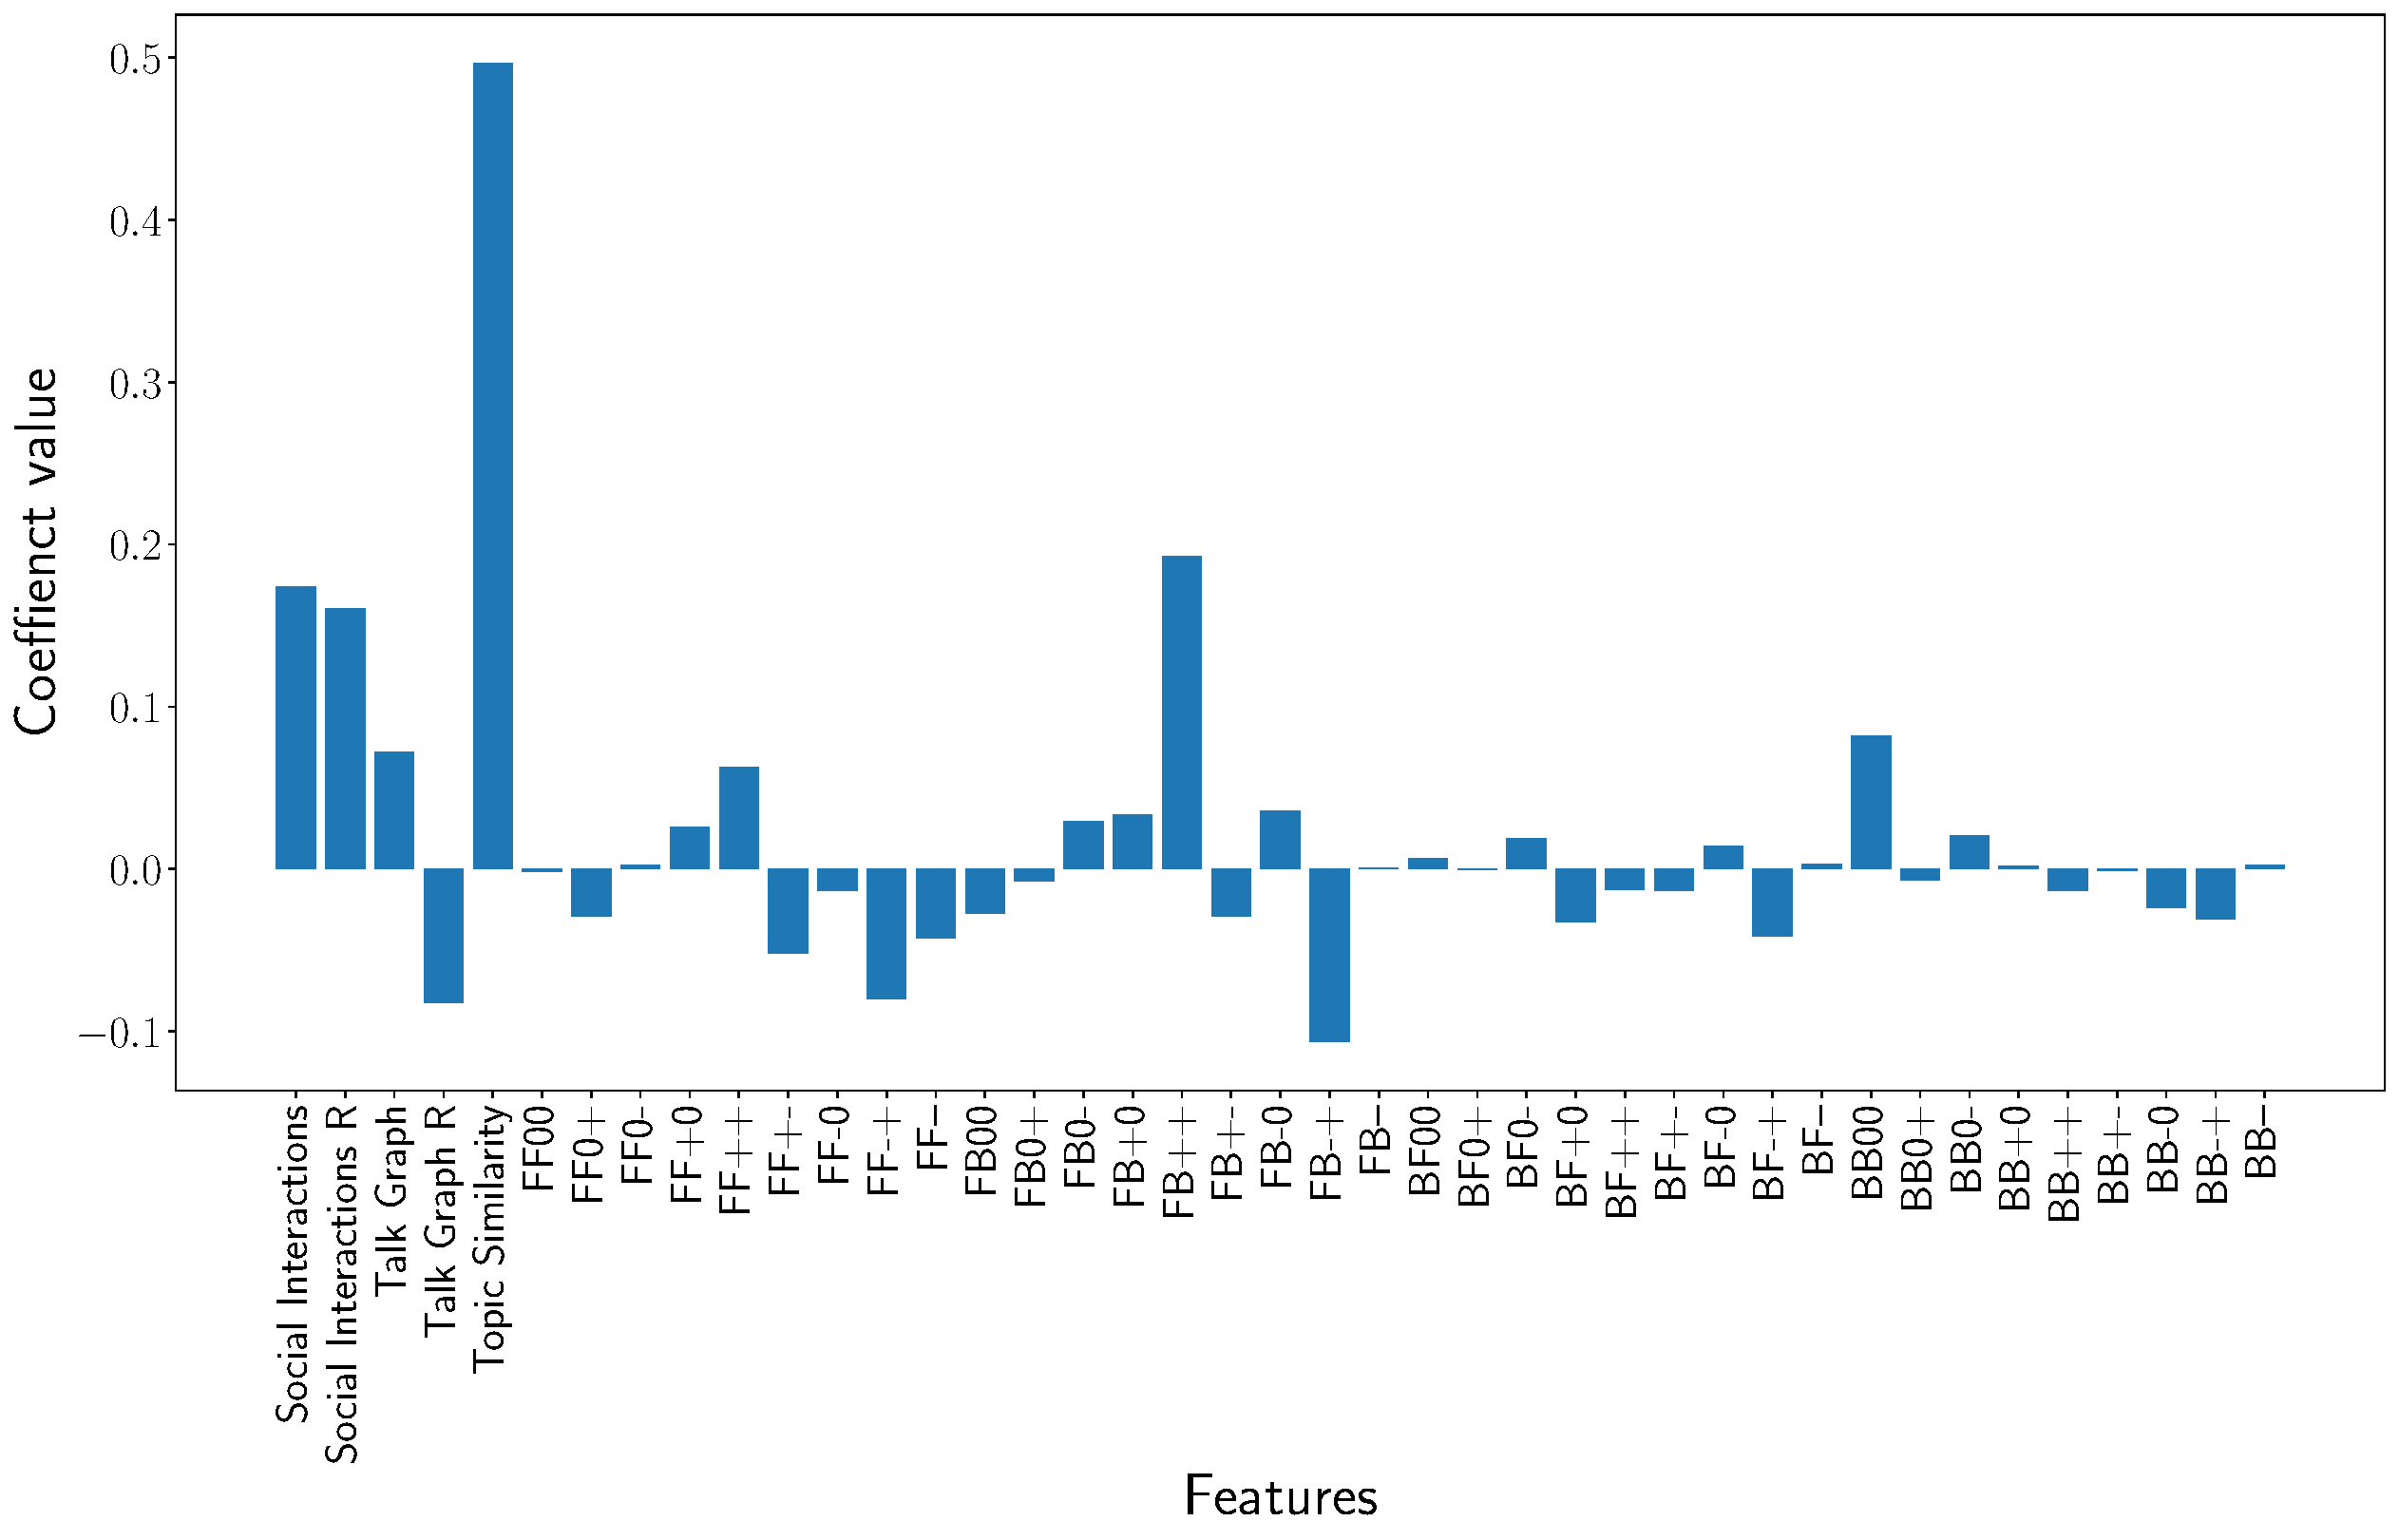
\includegraphics[width=\textwidth]{images/Logistic Regression_features.pdf}
    \caption{Feature importances of the trained Logistic Regression model }
    \label{fig:lr-feature-importances}
\end{figure}


Then, we tested the trained LR model on the test feature matrix and evaluated the output with the target vectors.
The results and the evaluation metrics are seen in Table~\ref{tab:test-results}.
We see that the graph combination model does not perform very well.
It has marginal gains on all three baseline metrics.
We can analyse these in more details looking at the ROC and PR curves, shown in Figure~\ref{fig:lr-test-plots}.
The ROC-AUC curve shows that model has a marginal improvement over the $0.5$ baseline.
Similarly, the \negPR curve depicts that the model fails to learn to predict negative votes more than the baseline of $0.2$. 
This combined with the marginal gain in predicting positive votes implies that the model has not learnt any statistically significant information.

We can explain the low performance of the model by using its lack of information.
As the features that are created for each vote are dependent on only the dev dataset, they have limited impact when predicting votes in the test dataset.
This is due to the fact that RfAs are chronological, as there are many more newer users in the test dataset and there is no information available on them in the dev dataset.
This problem might reduce, if we change the percentage of data in the dev, train and test datasets.
However, increasing the size of dev dataset split, leads to a lack of training data.
In this scenario, the LR model cannot efficiently learn the coefficients from the features that have now possess more information.
This leads again to the model only achieving marginal improvements over the baselines.

\begin{figure}[htp]
    \centering
    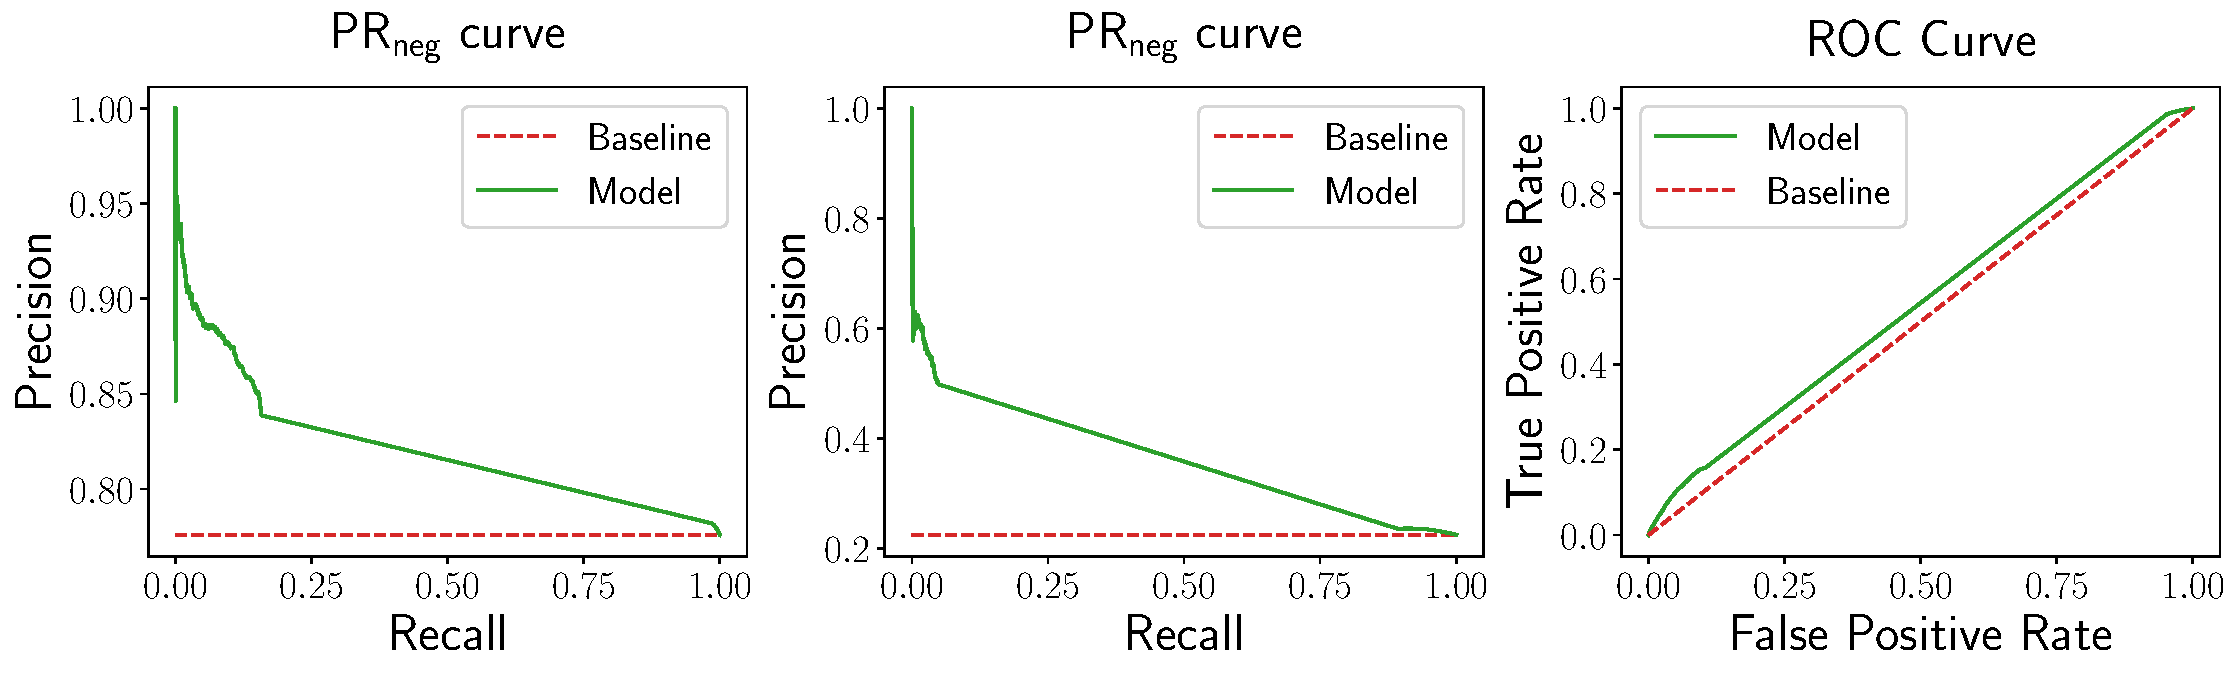
\includegraphics[width=\textwidth]{images/Logisitc Regression_test.pdf}
    \caption{Logistic Regression plots for test data}
    \label{fig:lr-test-plots}
\end{figure}

\subsection{Iterative Model Results}
Now, we discuss the results of the iterative models for the test dataset.
We see the evaluation metrics for both the iterative balance and status models in Table~\ref{tab:test-results}.
These results are the predictions the iterative models makes for the RfAs present in the test dataset. 
We see that both models perform much better than the baselines as well as the graphical combination model.

However, directly comparing the iterative models' result to the graphical model's result is not fair.
Because, the iterative models assimilate the information each election as they progress in the test dataset and utilize that information to predict votes in the next RfA.
Therefore, the predictions of the iterative model are not independent.
In spite of this, analysing the improvements of the iterative models provides understanding of the inherent shortcomings of the graphical combination model discussed previously.

Out of both models, we see that the \textit{Iterative Balance Model} performs much better.
We see that the model is able to better predict both positive and negative votes, seen by the large \aucposPR and \aucnegPR scores respectively.
This is in line with the previous analysis that balance theory better predicts triads in the voting neighbourhood.
Here, we see that the LSN of the voter conforms more according to balance theory than status theory. 

Another analysis, both the iterative balance and status models achieve better performance than the graphical combination model utilizing only the voting data.
Furthermore, this indicates that there is a scope of incorporating the auxiliary features to the iterative models to further improve the performance of the models.
Moreover, it clearly shows that solving the lack of information problem present in the graph combination model can lead to better predictions.

We can analyse the iterative models further considering the complete \wikirfa dataset.

\section{Complete \wikirfa Results}
\label{sec:complete-reults}
The iterative models described in Second~\ref{sec:local-signed-network-implementation}, can be bootstrapped to predict all the votes in the \wikirfa dataset.
The results for the models along with the baselines are shown in Table~\ref{tab:complete-results}.
We see the complete dataset is more imbalanced than the test dataset, seen by the larger \aucposPR and smaller \aucnegPR baselines.

\subsection{New Voter Analysis}
As discussed in Section~\ref{sec:local-signed-network-implementation}, we marked all votes that were predicted without any information when we encountered new voters.
This amounted to $11812$ or approximately $5.7\%$ of all votes predicted.
The distribution of the true value of these votes is $9217$ support and $2595$ oppose votes.
This shows that new voters are almost 3x more likely to vote positively.
We analysed these new voters' votes with the progress of the election of the time to study herd mentality.
Comparing these votes to the sign of the cumulative sum of votes until that point, we see that nearly 81\% of new votes are the same as the herd.
Similarity, we also compare the new voters to the votes cast by the person immediately before them.
We see that 76\% of new voters  agree with the previous voter.
Therefore, we can adopt a simple strategy of predicting the new voters to have a probability of voting support equal to the fraction of support votes cast until that point.

\begin{table}[htp]
    \centering
    \caption{Results of iterative models on the complete \wikirfa dataset}
    \label{tab:complete-results}
    \begin{tabular}{lccc}
        \toprule
        Model & AUC-ROC & \aucposPR  & \aucnegPR \\ 
        \midrule
        
        Baseline & 0.5 & 0.784& 0.216 \\

        Iterative Balance &  0.835 & 0.935 & 0.635 \\

        Iterative Status & 0.784 & 0.917 & 0.502 \\
        
        \bottomrule
        \end{tabular}
\end{table}

\begin{table}[htp]
    \centering
    \caption{Information of relationship graphs of iterative models using entire \wikirfa dataset}
    \label{tab:iterative-graphs}
    \begin{tabular}{lcccc}
        \toprule
        Relationship Graph & $|V|$ & $|E|$ & density & \shortstack{largest component \\size}\\
        \midrule
        
        Agreement Graph& 11924 &2451028 & 0.0345 & 11908\\
        
        Follow Graph & 11924 & 3136303 & 0.0220 & 11563 \\


        \bottomrule
        \end{tabular}
\end{table}

\subsubsection{Iterative Balance Model Results}
The iterative balance models performs very well even when predicting all the votes in the entire \wikirfa dataset.
The results in Table~\ref{tab:complete-results}, shows that on every metric the balance model has a significant margin over the baseline.
Especially, we see that negative votes are predicted almost three times better than the baseline, seen by the \aucnegPR score of $0.635$.
This indicates that the model has collected useful information in the \textit{agreement graph}, as seen in Table~\ref{tab:iterative-graphs}.
The graph obtained at the end of the process is fairly large and dense and is nearly connected.
Therefore, a rich representation of relationships between Wikipedia users is stored in the agreement graph.

\begin{figure}[htp]
    \centering
    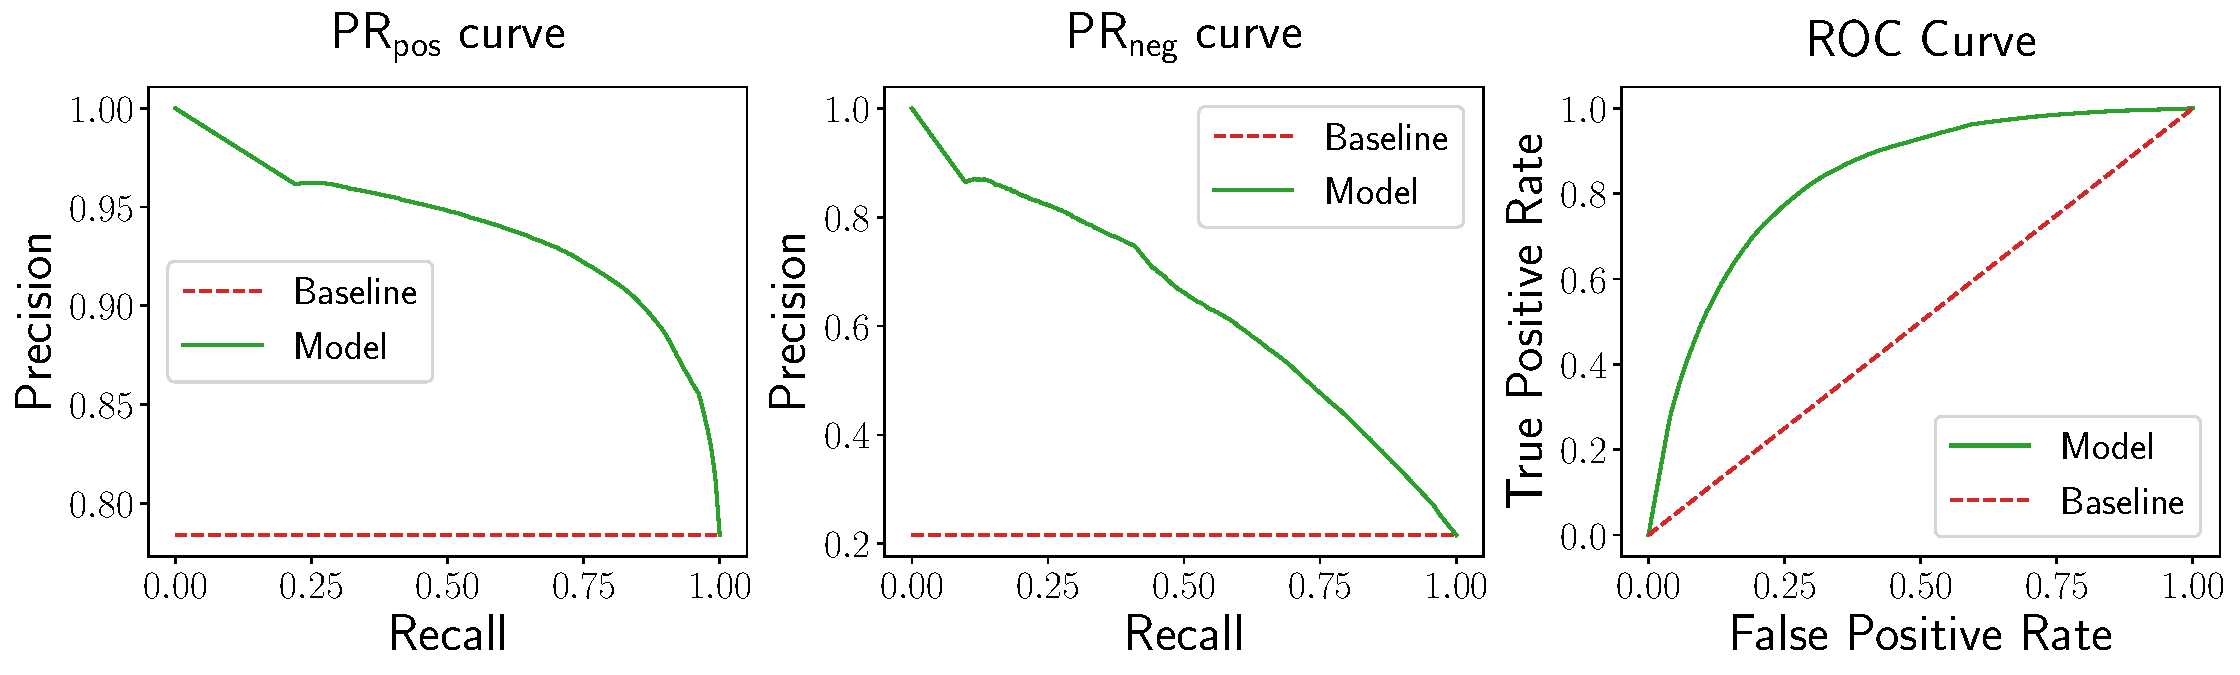
\includegraphics[width=\textwidth]{images/iterative_Balance.pdf}
    \caption{Plots for the Iterative Balance Model on the complete \wikirfa dataset}
    \label{fig:complete-iterative-balance}
\end{figure}
The plots in Figure~\ref{fig:complete-iterative-balance}, show that the model consistently performs well above the baselines.
Now, in choosing an optimal threshold for the model, we turn to the plots in Figure~\ref{fig:complete-iterative-balance-f1}.
These show how the F1 score changes as we move the threshold parameter $\theta$.
We see that the \posF score only starts to decrease gradually after $\theta=0.5$.
Also, there is a peak for the \negF score a little after the point of $\theta=0.5$.
Therefore, we can choose $\theta=0.53$, to obtain a \posF = 0.887 and \negF=0.602.
This gives us \macroF $= (0.887+0.602)/2 = 0.745$.
This threshold also indicates that even if $\lambda_{1}^{+}$ of the LSN is slightly smaller than $\lambda_{1}^{-}$ then the vote predicted is positive.
Therefore, the model has good compliance with balance theory.
\begin{figure}[htp]
    \centering
    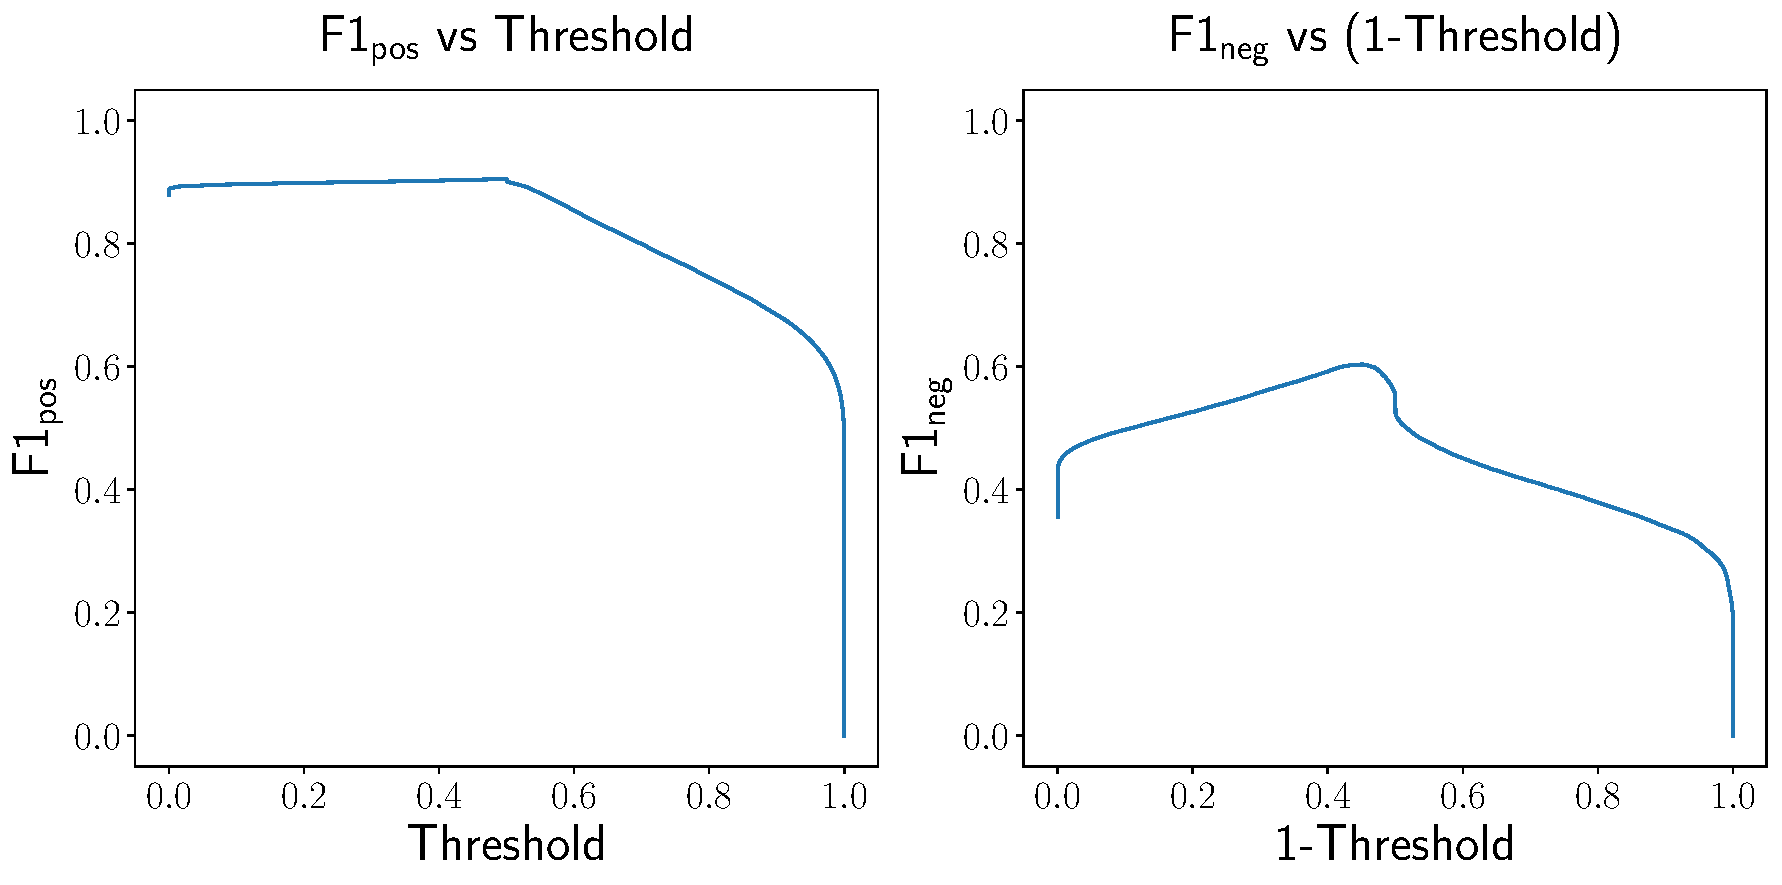
\includegraphics[width=0.75\textwidth]{images/iterative_Balance_f1.pdf}
    \caption{F1 score versus threshold plots for Iterative Balance Model}
    \label{fig:complete-iterative-balance-f1}
\end{figure}

\subsection{Iterative Status Model Results}
Table~\ref{tab:complete-results} show that the iterative status model also performs admirably above the baseline results.
We also see in Table~\ref{tab:iterative-graphs}, that the \textit{follow graph} is large, fairly dense and has large strongly connected components.
However, its performance is still relatively lower than the iterative balance model.

In Figure~\ref{fig:complete-iterative-status}, we see that the \posPR curve is nearly identical to that of the iterative balance model.
This is also reflected in the high \aucposPR score comparable to the iterative balance model.
However, the \negPR curve clearly shows that there is a lower quality when predicting negative votes.
This translates in the smaller \aucnegPR score and explains the overall lower AUC-ROC score of the model.
The lower predictive performance can be explained using our earlier analysis of the graph combination model.
We see that in reality, the triads where status theory is ambivalent actually have a preference for a particular sign.
Therefore, the cases when the agony of the LSN is equal for both cases, i.e., $\alpha^{+}=\alpha^{-}$, should not map to $p=0.5$.
Rather, we must modify status theory to better represent signed relationships in a network.

\begin{figure}[htp]
    \centering
    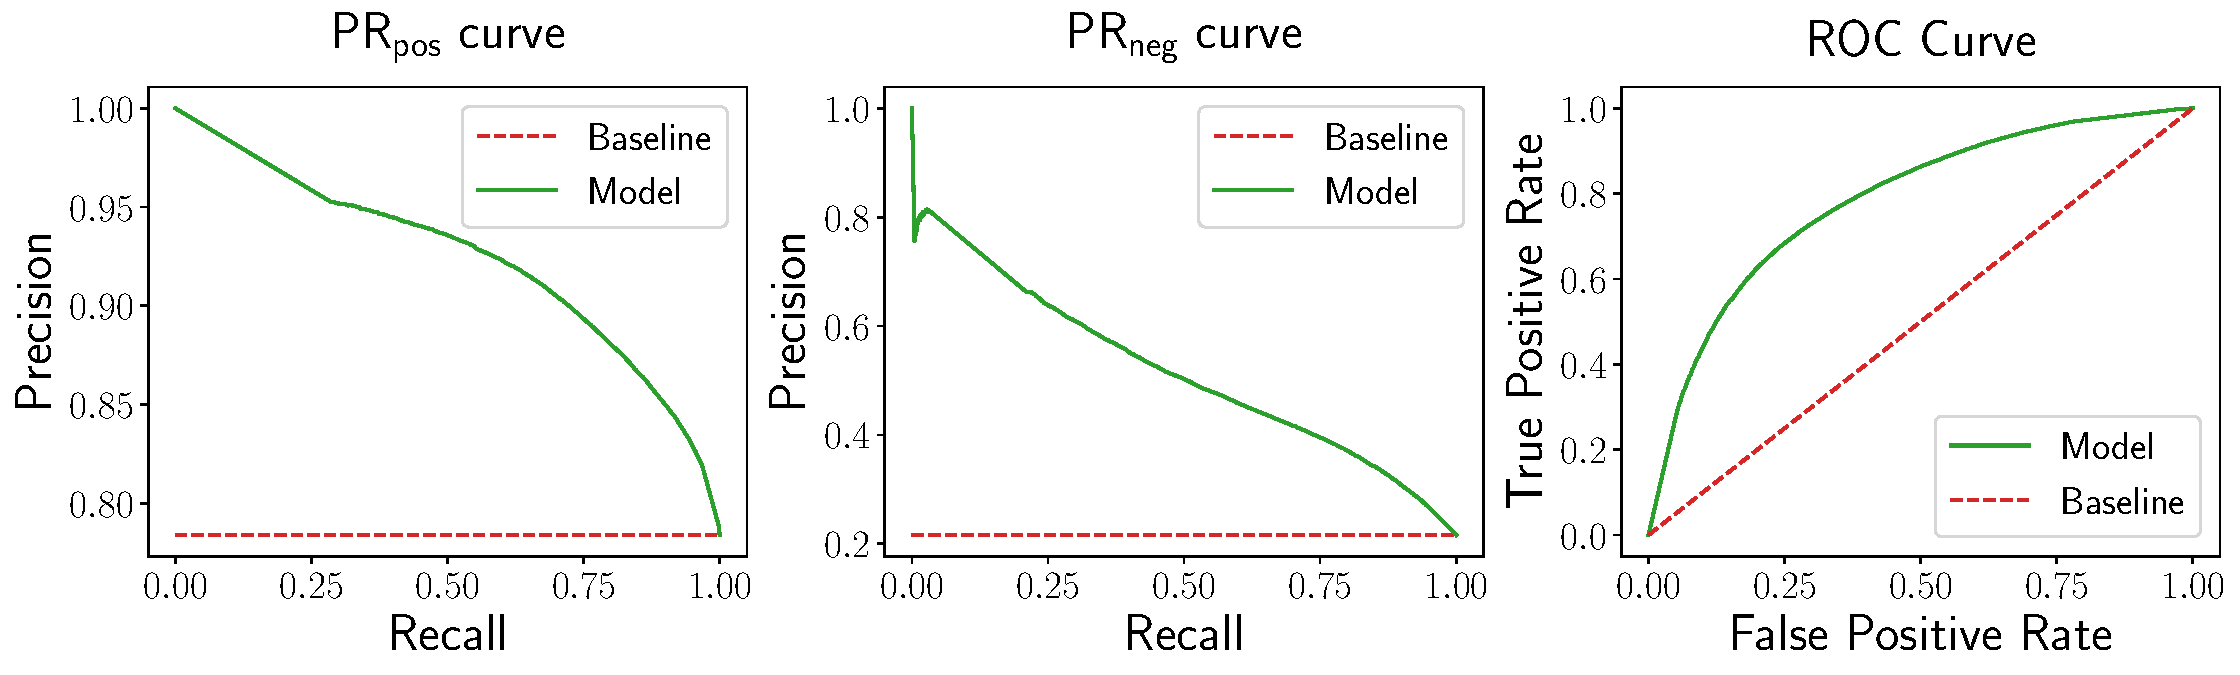
\includegraphics[width=\textwidth]{images/iterative_Status.pdf}
    \caption{Plots for the Iterative Status Model on the complete \wikirfa dataset}
    \label{fig:complete-iterative-status}
\end{figure}

In Figure~\ref{fig:complete-iterative-status-f1}, we see another issue caused by the large number of the support vote probabilities being 0.5.
The \posF curve is again identical to the \posF curve of the iterative balance model.
However, the \negF curve shows that there is an inflection at $\theta=0.5$.
The change is quite drastic with \negF$=0.05$ at $\theta=0.49$ and \negF$=0.32$ at $\theta=0.5$. 
This affects the choice of an optimal threshold for the model.
We see that the \negF score increases as threshold is increased beyond $\theta=0.5$.
This indicates that closer to 0.5, there are many false positives.
However, choosing $\theta=0.75$ at the peak of the \negF score is not suitable, as the \posF score starts to drop much more significantly. 
Hence, we choose $\theta=0.63$ as the constrained optimum giving us \posF=0.861 and \negF=0.504, therefore, \macroF = 0.606. 
This deterministic metric is also lower than the $0.745$ of the iterative balance model.
The choice of threshold close ot $=0.6$ suggests that the $\alpha^{+}$, the agony for the positive vote case, must be considerably lower than $\alpha^{-}$, the agony for the negative vote case, to predict a positive vote.
Therefore, this also indicates that we need to make additional modifications to status theory if we want to increase the predictive power of the iterative status model.


\begin{figure}[htp]
    \centering
    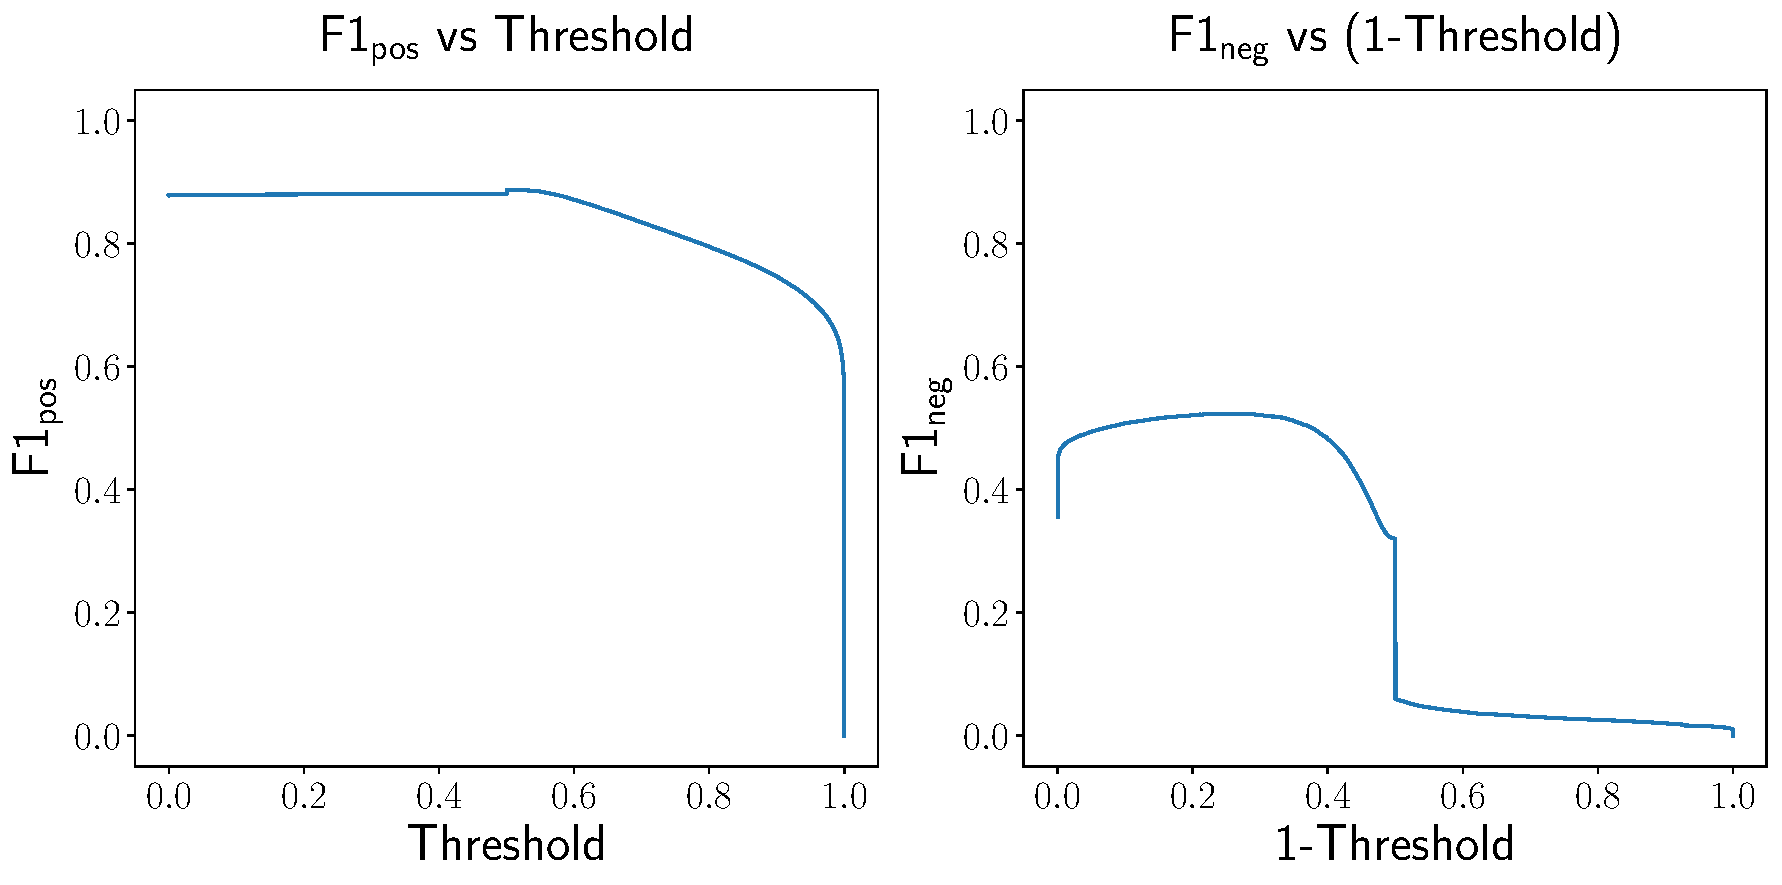
\includegraphics[width=0.75\textwidth]{images/iterative_Status_f1.pdf}
    \caption{F1 score versus threshold plots for Iterative Status Model}
    \label{fig:complete-iterative-status-f1}
\end{figure}


\section{Voting Order Results}
\label{sec:voting-order-results}
In Section~\ref{sec:voting-order}, we discussed how to study the effects of voting order on the performance of the iterative models trained on the complete \wikirfa dataset.
The results for the third RfA nomination  of user \textit{Hawkeye7} is presented in Table~\ref{tab:fail-rfa} and is referred to the \textit{failed RfA}.
Similarly, the results of user \textit{HickoryOughtShirt?4}'s nomination is show in table~\ref{tab:pass-rfa} and is called the \textit{successful RfA}.

\subsection{Failed RfA Results}
We see that the voting in the failed RfA is fairly tight.
The \aucposPR score is 0.52 and \aucnegPR is 0.479, indicating that the election did indeed have more support votes than oppose.
Nevertheless, the RfA failed as the Bureaucrat responsible concluded that the consensus was to not promote the user.

For the \textit{normal voting order}, as seen in Table~\ref{tab:fail-rfa}, the balance model performs much worse when compared to the status model.
In fact, the iterative balance model performs below the baseline for all metrics.
This can be attributed to the fact that this particular user had two previous nominations of which one was successful.
Therefore, a symmetric measure of agreement might not be helpful in predicting the balance as the election progresses, especially when the voting margins are tight.
On the other hand, we see that the iterative status model performs better the iterative balance model, but is still worse than the baseline metrics for a random model.
This clearly shows that both models are struggling to predict votes in a RfAs with a narrow margin of difference between support and oppose votes.  

For the \textit{reversed voting order}, we see that iterative balance model performs considerably better compared to the normal voting order.
Especially, we see that all the metrics, i.e., AUC-ROC, \aucposPR and \aucnegPR scores have improved above the baseline, increasing the model's overall performance.
This is interesting, as it suggests that the LSNs formed by reversing the voting order provides better information on the voting behaviour than the actual voting order.
Similarly, we see the status model also gaining in performance when the voting order is reversed.
Although the \aucnegPR score is still below the baseline, we see the overall performance has improved.
We can explain the model's difficulty in predicting negative votes using our previous analysis; status theory complies less with the true data than balance theory.
Therefore, we infer that reversing the voting order improves the performance of both models.

Meanwhile, the results of the average of ten \textit{random voting orders} for both models lie in between the results for the normal and reversed voting methods.
We see that the result for the iterative balance model is above the baseline for all metrics and the iterative status model is close to the baseline.
Therefore, we see that the voting order does affect the performance of the iterative models and that we can benefit from reversing the voting order and averaging the results to obtain better predictions for RfAs that have tight margins. 

\begin{table}[htp]
    \centering
    \caption{Results for different vote orderings for the failed RfA}
    \label{tab:fail-rfa}
    \begin{tabular}{llccc}
        \toprule
        Model & Vote Order & AUC-ROC & \aucposPR  & \aucnegPR \\ 
        \midrule
        
        Baseline & - & 0.5 & 0.52 & 0.479 \\
        \midrule
        
        \multirow{3}{*}{\shortstack[l]{Iterative\\ Balance}} & 
        Normal &  0.392 & 0.490 & 0.403 \\
        % \cmidrule{2-5}
        &Reversed & 0.575 & 0.606 & 0.529 \\
        % \cmidrule{2-5}
        & Random & 0.527 & 0.552 & 0.517 \\
        \midrule

        \multirow{3}{*}{\shortstack[l]{Iterative\\ Status}} & 
        Normal & 0.454 & 0.532 & 0.457 \\
        % \cmidrule{2-5}
        & Reversed & 0.515 & 0.563& 0.466   \\
        % \cmidrule{2-5}
        & Random & 0.493 & 0.538 & 0.480 \\
        \bottomrule
        \end{tabular}
\end{table}

\subsection{Successful RfA Results}
In Table~\ref{tab:pass-rfa}, we see that the result of the RfA is clearly evident in the \aucposPR and \aucnegPR baselines.
Nearly, all votes are supporting the candidate and there are a few minority opposition votes. 
For this RfA, we see the results are in line with the results we obtained for the failed RfA.

For the \textit{normal voting order}, we see that the iterative balance model has AUC-ROC and \aucposPR scores lower than the baseline but \aucnegPR scores well above the baseline.
This indicates that the model is better able to predict oppose votes, but at the cost of the better predictions for the support votes. 
We see a similar phenomenon for the iterative status model where the \aucposPR is below the baseline but the overall AUC-ROC is slightly above the random model baseline.
This highlights the difficulty of predicting the oppose votes in a fairly clear election.

Once again, in the results for the \textit{reversed voting order}, we see that both iterative models have better performance across all metrics.
Especially, we see both models have much larger \aucposPR scores which in turn boosts the AUC-ROC scores, as the positive votes are the majority in this RfA.
As a result, we also see that the \aucnegPR scores drop, indicating the tension in optimizing both positive and negative vote prediction.

The average of 10 \textit{random voting order} results show that the performance of the models are overall better than the normal voting order.

A note to consider is that this analysis and results are only for the two new RfAs and can be further analysed in detail as a separate project.
\begin{table}[htp]
    \centering
    \caption{Results for different vote orderings for the successful RfA}
    \label{tab:pass-rfa}
    \begin{tabular}{llccc}
        \toprule
        Model & Vote Order & AUC-ROC & \aucposPR  & \aucnegPR \\ \midrule
        Baseline & - & 0.5 & 0.905 & 0.095 \\
        \midrule
        
        \multirow{3}{*}{\shortstack[l]{Iterative\\ Balance}} & 
        Normal &  0.48 & 0.90 & 0.231 \\
        % \cmidrule{2-5}
        &Reversed & 0.649 & 0.933 & 0.216 \\
        % \cmidrule{2-5}
        & Random & 0.607 & 0.921 & 0.273 \\
        \midrule
        
        \multirow{3}{*}{\shortstack[l]{Iterative\\ Status}} & 
        Normal & 0.503 & 0.898 & 0.211 \\
        % \cmidrule{2-5}
        & Reversed & 0.628 & 0.931 & 0.151 \\
        % \cmidrule{2-5}
        & Random & 0.612 & 0.921 & 0.230 \\
        \bottomrule
        \end{tabular}
\end{table}



